% !TEX root = Projektdokumentation.tex
\section{Anhang}
\subsection{Detaillierte Zeitplanung}
\label{app:Zeitplanung}

\tabelleAnhang{ZeitplanungKomplett}

\subsection{Übersicht Ressourcenplanung}
\label{app:Ressourcenplanung}

\tabelleAnhang{Ressourcenplanung}

\subsection{Lastenheft (Auszug)}
\label{app:Lastenheft}
Es folgt ein Auszug aus dem Lastenheft mit Fokus auf die Anforderungen:

Die Anwendung muss folgende Anforderungen erfüllen:
\begin{enumerate}[itemsep=0em,partopsep=0em,parsep=0em,topsep=0em]
    \item Generierung und Verwaltung von QR-Codes
    \begin{enumerate}
        \item Die Anwendung muss für jede abgeschlossene Bestellung einen einzigartigen QR-Code generieren.
        \item Es muss ein Eintrag für jedes Ticket in die Datenbank geschrieben werden.
        \item Die QR-Codes müssen per E-Mail an die Kunden versendet werden.
    \end{enumerate}

    \item Einlösung und Verifizierung von QR-Codes
    \begin{enumerate}
        \item Die Anwendung muss das Scannen der QR-Codes ermöglichen.
        \item Die Anwendung muss die Gültigkeit der gescannten QR-Codes überprüfen.
        \item Die Anwendung muss die Bestellinformationen anzeigen, wenn ein QR-Code gescannt wird.
        \item Die Anwendung muss es ermöglichen, die Einlösung der QR-Codes zu bestätigen und diese als eingelöst zu markieren.
        \item Ungültige oder bereits eingelöste QR-Codes dürfen nicht erneut akzeptiert werden.
    \end{enumerate}

    \item Benutzeroberfläche und Usability
    \begin{enumerate}
        \item Die Benutzeroberfläche muss intuitiv und benutzerfreundlich gestaltet sein.
        \item Die Navigation durch die Anwendung muss einfach und klar strukturiert sein.
        \item Fehlermeldungen müssen verständlich und hilfreich sein, um dem Benutzer bei der Problembehebung zu helfen.
    \end{enumerate}

    \item Sicherheit und Zugriffskontrolle
    \begin{enumerate}
        \item Die Anwendung muss vor gefälschten und manipulierten QR-Codes sicher sein.
        \item Es muss sichergestellt werden, dass nur autorisierte Mitarbeiter mit einem hinterlegten Login Zugang zur Anwendung haben.
        \item Die Zugriffskontrolle muss verhindern, dass unbefugte Personen sensible Bestellinformationen einsehen oder Tickets versehentlich entwerten können.
    \end{enumerate}

    \item Integrationsfähigkeit
    \begin{enumerate}
        \item Die Anwendung muss sich nahtlos in die bestehende Systemlandschaft integrieren.
        \item Die Struktur der Anwendung muss den Anforderungen eines Symfony Bundles entsprechen.
    \end{enumerate}

    \item Zuverlässigkeit und Effizienz
    \begin{enumerate}
        \item Die Anwendung muss verlässlich und korrekt arbeiten.
        \item Kritische Fehler, die das gesamte Programm lahmlegen, müssen unbedingt vermieden werden.
    \end{enumerate}
\end{enumerate}


\clearpage

\subsection{Use Case-Diagramm}
\label{app:UseCase}

\includegraphicsKeepAspectRatio{Bilder/UseCaseFinish.png}{1}

\subsection{Pflichtenheft (Auszug)}
\label{app:Pflichtenheft}

\subsubsection*{Zielbestimmung}

\begin{enumerate}[itemsep=0em,partopsep=0em,parsep=0em,topsep=0em]
    \item \textbf{Generierung und Verwaltung von QR-Codes}
    \begin{enumerate}
        \item Das Programm wird eine Funktion zur automatischen Generierung eines einzigartigen QR-Codes für jede abgeschlossene Bestellung implementieren.
        \item Die QR-Codes werden mithilfe einer Bibliothek namens \texttt{php-qrcode} erstellt. Diese Bibliothek ermöglicht es eine Zeichenkette in einen QR-Code zu verwandeln.
        \item Jeder generierte QR-Code wird in der Datenbank gespeichert. Dazu wird eine Tabelle \texttt{tl\_iso\_order\_hashes} verwendet, die die QR-Codes zusammen mit der zugehörigen Bestell-ID und weiteren Metadaten speichert.
        \item Die generierten QR-Codes werden automatisch per E-Mail an die Kunden versendet. Dafür wird eine E-Mail-Versandfunktion integriert, die die QR-Codes als Anhang oder Bild in die E-Mail einfügt.
    \end{enumerate}
    
    \item \textbf{Einlösung und Verifizierung von QR-Codes}
    \begin{enumerate}
        \item Das Programm wird eine Scanfunktion bereitstellen, die mithilfe der Bibliothek \texttt{html5-qrcode} die QR-Codes mit der Kamera eines mobilen Endgeräts scannt.
        \item Die Gültigkeit der gescannten QR-Codes wird überprüft, indem der QR-Code mit den in der Datenbank gespeicherten Hashes abgeglichen wird. Es wird sichergestellt, dass der QR-Code gültig und nicht bereits eingelöst ist.
        \item Nach dem Scannen eines QR-Codes zeigt das Programm die relevanten Bestellinformationen an, die aus der Datenbank abgerufen werden. Diese Informationen umfassen die Bestellnummer, den Namen des Kunden und die Details der Bestellung.
        \item Die Einlösung der QR-Codes wird im System markiert, indem der Status des QR-Codes in der Datenbank auf "eingelöst" gesetzt wird. Dies verhindert die erneute Nutzung des gleichen QR-Codes.
        \item Das Programm stellt sicher, dass ungültige oder bereits eingelöste QR-Codes nicht akzeptiert werden, indem es eine entsprechende Fehlermeldung anzeigt.
    \end{enumerate}

    \item \textbf{Benutzeroberfläche und Usability}
    \begin{enumerate}
        \item Die Benutzeroberfläche wird mithilfe von HTML5-Templates und SCSS entwickelt. Diese Templates werden so gestaltet, dass sie intuitiv und benutzerfreundlich sind.
        \item Die Navigation innerhalb des Programms wird klar und logisch strukturiert, sodass Benutzer leicht zwischen den verschiedenen Funktionen wechseln können.
        \item Fehlermeldungen werden klar formuliert und hilfreich gestaltet, um den Benutzern die Lösung von Problemen zu erleichtern. Für das anzeigen dynamischer Fehlermeldungen wird JavaScript verwendet.
    \end{enumerate}

    \item \textbf{Sicherheit und Zugriffskontrolle}
    \begin{enumerate}
        \item Das Programm wird Maßnahmen zum Schutz vor gefälschten und manipulierten QR-Codes integrieren.
        \item Es wird sichergestellt, dass nur autorisierte Mitarbeiter Zugang zum Programm haben. Dies wird durch die Mitgliedsverwaltung in Contao realisiert, die den Zugriff auf bestimmte Funktionen und Daten einschränkt.
        \item Die Zugriffskontrolle verhindert, dass unbefugte Personen sensible Bestellinformationen einsehen oder Tickets versehentlich entwerten können.
    \end{enumerate}

    \item \textbf{Integrationsfähigkeit}
    \begin{enumerate}
        \item Das Programm wird als Symfony Bundle entwickelt, das sich nahtlos in die bestehende Contao-Umgebung integrieren lässt. Dies erleichtert die Installation und Wartung.
        \item Die Struktur des Programms entspricht den Anforderungen eines Symfony Bundles, sodass es problemlos in andere Projekte eingebunden werden kann.
    \end{enumerate}

    \item \textbf{Zuverlässigkeit und Effizienz}
    \begin{enumerate}
        \item Das Programm wird so entwickelt, dass es zuverlässig und korrekt arbeitet. Dies wird durch manuelle Frontend-Tests sichergestellt.
    \end{enumerate}
\end{enumerate}

\subsubsection*{Produkteinsatz}

\begin{enumerate}[itemsep=0em,partopsep=0em,parsep=0em,topsep=0em]
    \item Anwendungsbereiche\\
    Das QR-Code-basierte Einlösungsprogramm dient zur Verwaltung und Verifizierung von Online-Tickets. Es soll eine effiziente und sichere Abwicklung der Ticketverkäufe und deren Einlösung vor Ort ermöglichen.

    \item Zielgruppen\\
    Die Hauptnutzer der Anwendung sind unsere Kunden, die für die Verifizierung und Einlösung der Tickets ihrer Online-Shops verantwortlich sind. Dazu gehören insbesondere Mitarbeiter in der Veranstaltungsbranche, im Einzelhandel sowie im Tourismusbereich.

    \item Betriebsbedingungen\\
    Die Anwendung muss auf Smartphones mit Webbrowser und Internetverbindung lauffähig sein. Das Programm wird als Webanwendung bereitgestellt. Eine ständige Verfügbarkeit der Anwendung ist durch den Betrieb auf einem Webserver sichergestellt. Updates und Wartungen werden zentral durchgeführt, um die kontinuierliche Verfügbarkeit zu gewährleisten.
\end{enumerate}

\subsection{Datenbankmodell}
\label{app:Datenbankmodell}

\begin{figure}[htb]
\centering
\includegraphicsKeepAspectRatio{Bilder/ERDProjektarbeitRework.png}{0.9}
\caption{Datenbankmodell}
\end{figure}
\clearpage
\subsection{Screenshots des Codes}
\label{ScreenhotsCode}

\subsubsection{DCA}
\label{app:ScreenshotDca}
\begin{figure}[htb]
\centering
\includegraphicsKeepAspectRatio{iso_order_hashes.pdf}{1}
\caption{Datenbankdefinition in iso\_order\_hashes.php}
\end{figure}
\clearpage
% \begin{figure}[htb]
% \centering
% \includegraphicsKeepAspectRatio{modulliste.pdf}{1}
% \caption{Liste der Module mit Filtermöglichkeiten}
% \end{figure}
% \clearpage

\subsection{Screenshots der Anwendung}
\label{Screenshots}
\begin{figure}[htb]
\centering
\includegraphicsKeepAspectRatio{tagliste.pdf}{1}
\caption{Anzeige und Filterung der Module nach Tags}
\end{figure}
\clearpage
\begin{figure}[htb]
\centering
\includegraphicsKeepAspectRatio{modulliste.pdf}{1}
\caption{Liste der Module mit Filtermöglichkeiten}
\end{figure}
\clearpage

\subsection{Entwicklerdokumentation}
\label{app:Doc}
\begin{center}
% Dokumentierte PHP-Funktionen
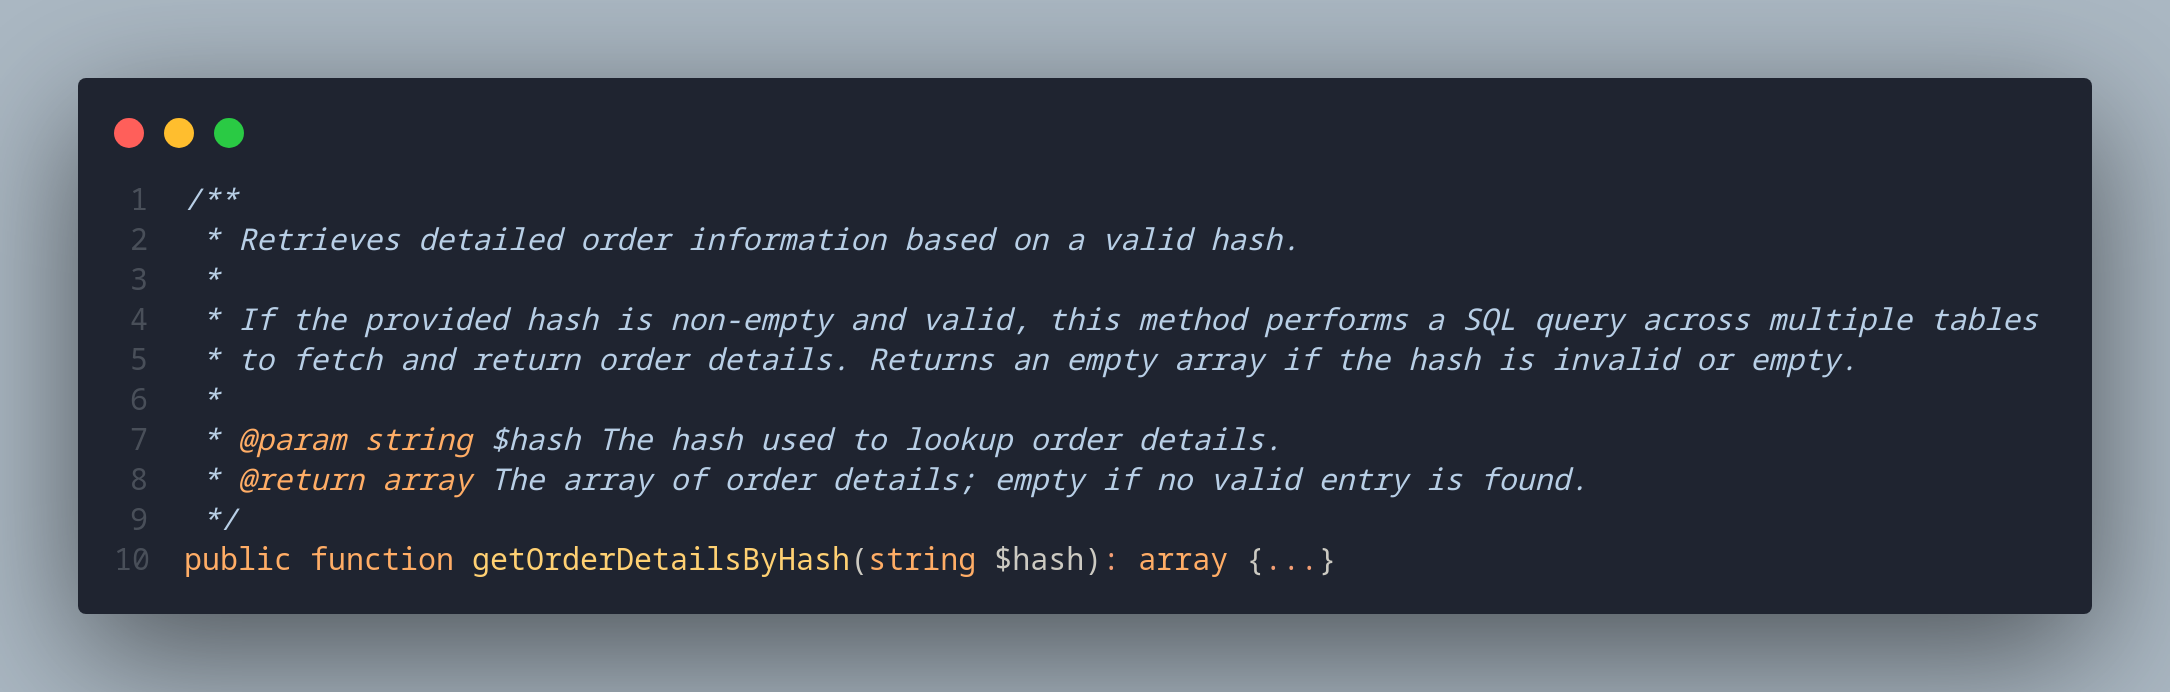
\includegraphics[page=1, width=1\textwidth]{getOrderDetailsByHash.png}
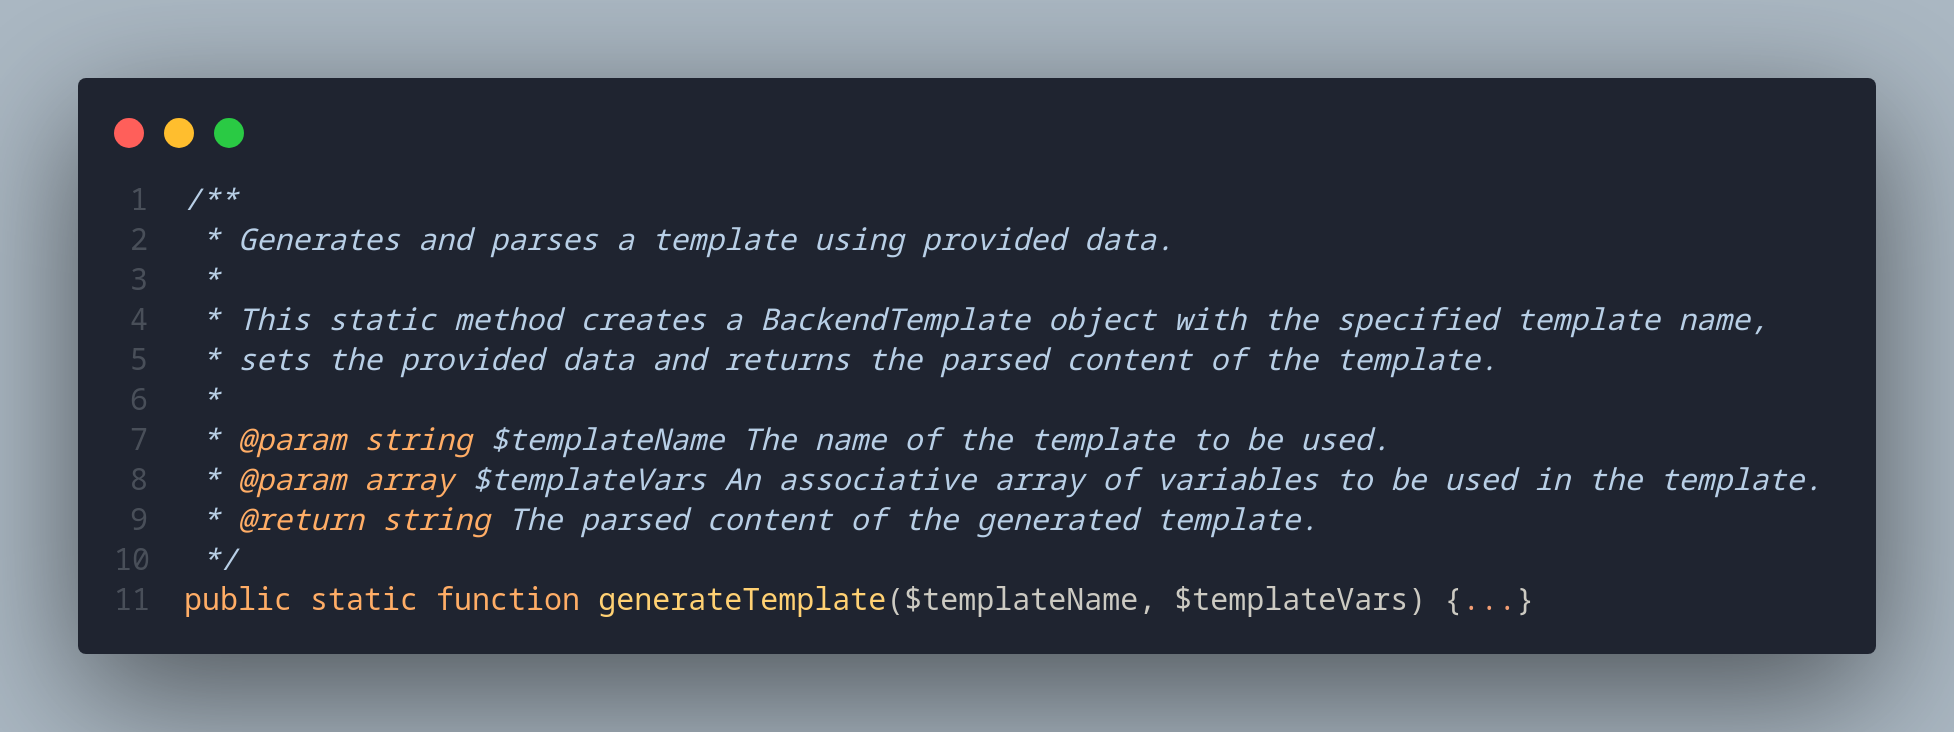
\includegraphics[page=1, width=1\textwidth]{generateTemplateHelper.png}
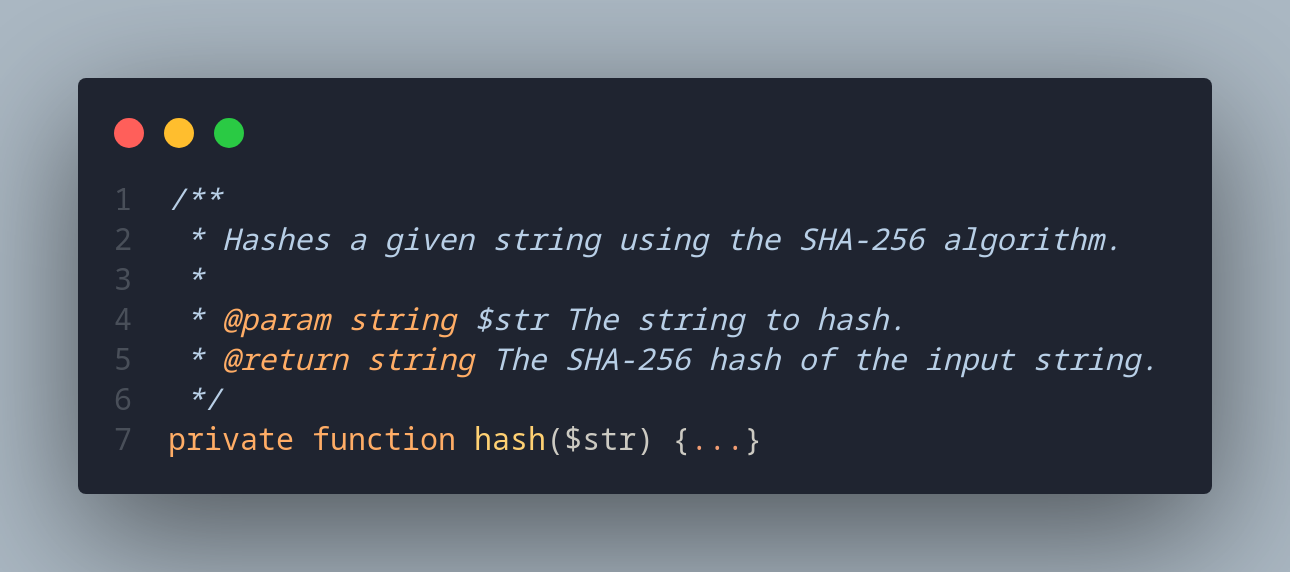
\includegraphics[page=1, width=1\textwidth]{hash.png}
\end{center}


\subsection{Testprotokoll}
\label{app:test}
\includegraphicsKeepAspectRatio{md/testprotokoll-1-1.png}{1}
\clearpage
\includegraphicsKeepAspectRatio{md/testprotokoll-2-1.png}{1}
\clearpage

\subsection{Klasse: TicketRoutes}
\label{app:CNMI}
Verkürzte Variante. Kommentare und Imports werden nicht angezeigt.
\lstinputlisting[language=php, caption={Klasse: TicketRoutes}]{Bilder/TicketRoutes.php}
\clearpage

\subsection{Klasse: TLOrderHashes}
\label{app:OrderHashes}
Verkürzte Variante. Kommentare und Imports werden nicht angezeigt.
\lstinputlisting[language=php, caption={Klasse: TLOrderHashes}]{Bilder/TLOrderHashes.php}
\clearpage

\subsection{Klassendiagramm}
\label{app:Klassendiagramm}
Klassendiagramme und weitere \acs{UML}-Diagramme kann man auch direkt mit \LaTeX{} zeichnen, siehe \zB \url{http://metauml.sourceforge.net/old/class-diagram.html}.
\begin{figure}[htb]
\centering
\includegraphicsKeepAspectRatio{Klassendiagramm.pdf}{1}
\caption{Klassendiagramm}
\end{figure}
\clearpage

\subsection{Benutzerdokumentation}
\label{app:BenutzerDoku}

\justifying

\subsubsection{Starten des Programms}
Öffnen Sie den Webbrowser Ihrer Wahl und navigieren Sie zu \url{https://[domain]/einloesen}. Wenn Sie nicht eingeloggt sind, dann werden Sie nun zur Login-Seite weitergeleitet. Melden Sie sich hier mit Ihrem Mitgliedszugang von Contao an.

Nachdem Sie sich erfolgreich eingeloggt haben, werden Sie zur Startseite weitergeleitet.

Stellen Sie sicher, dass Ihre Kamera und Internetverbindung aktiviert sind, um alle Funktionen der Anwendung nutzen zu können.

\subsubsection{Scannen eines QR-Codes}
\textbf{QR-Code-Scanner öffnen:} Klicken sie auf der Startseite auf das QR-Code-Icon um den Scan-Prozess zu starten.

\textbf{Kamera ausrichten:} Richten Sie die Kamera Ihres Geräts auf den QR-Code des Tickets. Achten Sie darauf, dass der QR-Code vollständig im Sichtfeld der Kamera ist.

\textbf{QR-Code scannen:} Das Programm scannt den QR-Code automatisch und leitet Sie zur Ticketinformation weiter. Hier sehen Sie alle relevanten Details zur Bestellung.


\subsubsection{Entwertung des Tickets}

Nachdem der QR-Code erfolgreich gescannt wurde, können Sie das Ticket entwerten:

\textbf{Ticketinformationen überprüfen:} Stellen Sie sicher, dass die angezeigten Informationen mit den Daten des Gastes übereinstimmen.

\textbf{Ticket entwerten:} Klicken Sie auf die Schaltfläche "Ticket entwerten", um den QR-Code im System als eingelöst zu markieren.


\subsubsection{Fehlerbehebung beim Scannen}

Sollte der Scan fehlschlagen, gibt es einige Ansätze, um das Problem zu beheben:

\textbf{Lichtverhältnisse anpassen:} Starkes Sonnenlicht kann den Bildschirm eines Handys schwer erkennbar machen. Stellen Sie sich, wenn nötig, in den Schatten, um den QR-Code besser sichtbar zu machen.

\textbf{QR-Code vergrößern:} Wenn der QR-Code zu klein dargestellt wird, können Sie den Bildschirm vergrößern, um den QR-Code besser erkennbar zu machen. Nutzen Sie die Zoom-Funktion Ihres Geräts.


\subsubsection{Manuelle Suche für Tickets}

Falls der Scan-Prozess gerade nicht funktioniert, haben sie die Möglichkeit manuell nach Tickets zu suchen. Hierbei kann nach Datum, Bestellnummer oder Name gesucht werden.

\textbf{Zur Ticketliste wechseln:} Klicken Sie auf der Hauptseite oder im QR-Code-Scanner auf den Button mit der Lupe, um zur Ticketliste zu gelangen.

\textbf{Ticketnummer eingeben:} Geben Sie die Ticketnummer, Datum oder den Namen des Gastes in die Suchleiste ein.

\textbf{Ticket entwerten:} Wählen Sie das entsprechende Ticket aus der Liste aus und klicken Sie auf "Ticket entwerten", um es manuell zu entwerten.


